\section*{Summary}
\renewcommand{\thefigure}{S-\arabic{figure}}

The parsimonious mixed member (PMM) model is a voting system designed such that:

\begin{itemize}
\item Every constituency is represented by a specific MP, and proportional seating ensures that no party is underrepresented. This is achieved with the smallest possible parliament size. 
\item Local races retain their importance, unlike in traditional mixed-member (MM).
\item Spoiled, and minor-party ballots are not misattributed to major parties (as is tacitly done in traditional MM). Voters have the right to vote for independent candidates and no party.
\item Changes to the current system are minimized and justified based on evidence of success in existing democracies.
\end{itemize}

To illustrate, projected results from the 2019 election are converted to quotients (see supplement) shown in Fig.~\ref{fig:sum_Qlist_byparty_2019}, along with an example threshold. Converting all data points above this line into seats would produce a 338-member legislature in proportion to popular vote. 
\begin{figure}[h!]
  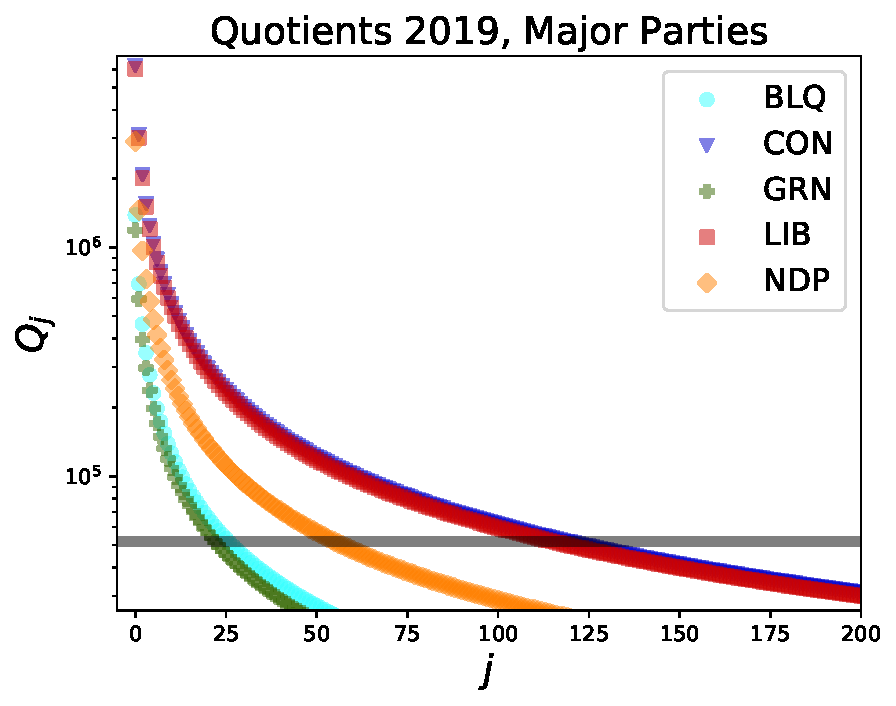
\includegraphics[width=0.50\textwidth,clip]{PR_calcs/data/raw_2019/PMM_out/PMM_Qlist_byparty.pdf}
%\captionsetup{labelformat=empty}
  \caption{`Quotients' from the 2019 Canadian popular vote. The grey threshold separates the largest 338 quotients, which can be converted into a proportional legislature. Ridings are incorporated in Fig.~\ref{fig:sum_Qlist_ordered_2019}. }
\label{fig:sum_Qlist_byparty_2019}
\end{figure}

Fig.~\ref{fig:sum_Qlist_ordered_2019} ensures a place for the local winners of each constituency while also determining the minimum necessary number of additional seats.
\begin{figure}
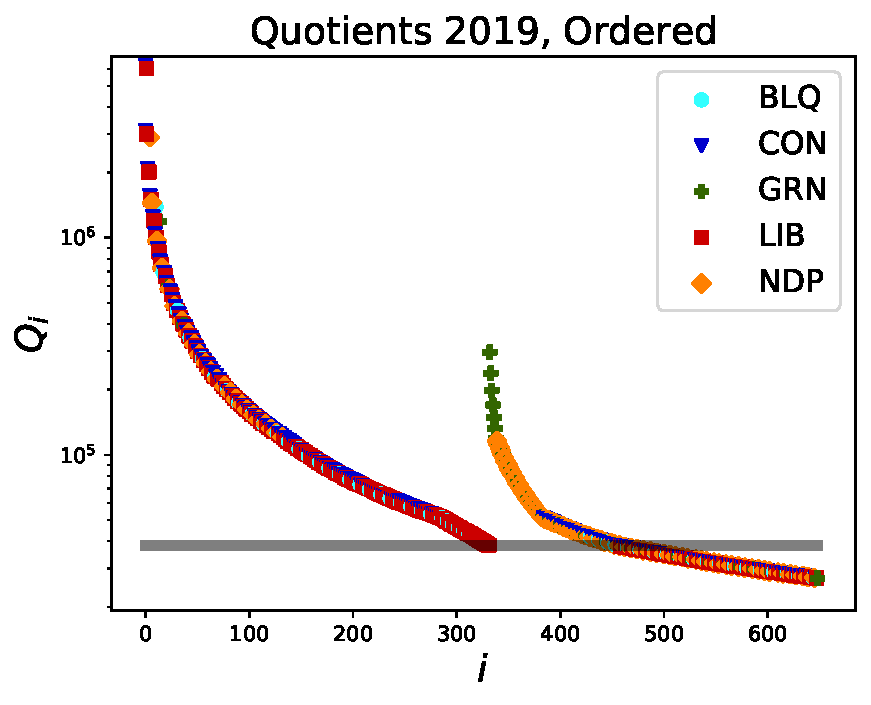
\includegraphics[width=0.50\textwidth,clip]{PR_calcs/data/raw_2019/PMM_out/PMM_Qlist_all.pdf}
\caption{ In PMM, quotients are ranked from all parties, giving priority to constituency seats (to the left), similar to the additional member system (AMS). However, the lowest-quotient from this group defines the threshold (horizontal, grey) for supplementary seats (right of the `jump' in this data). Quotients below this threshold are generally ignored (whereas traditional MM would convert all quotients shown to a seat.)}
\label{fig:sum_Qlist_ordered_2019}
\end{figure}
Finally, Fig.~\ref{fig:sum_projection_2019} projects the change in standings in parliament with PMM. Further details and examples are provided in the main text.

\begin{figure}
  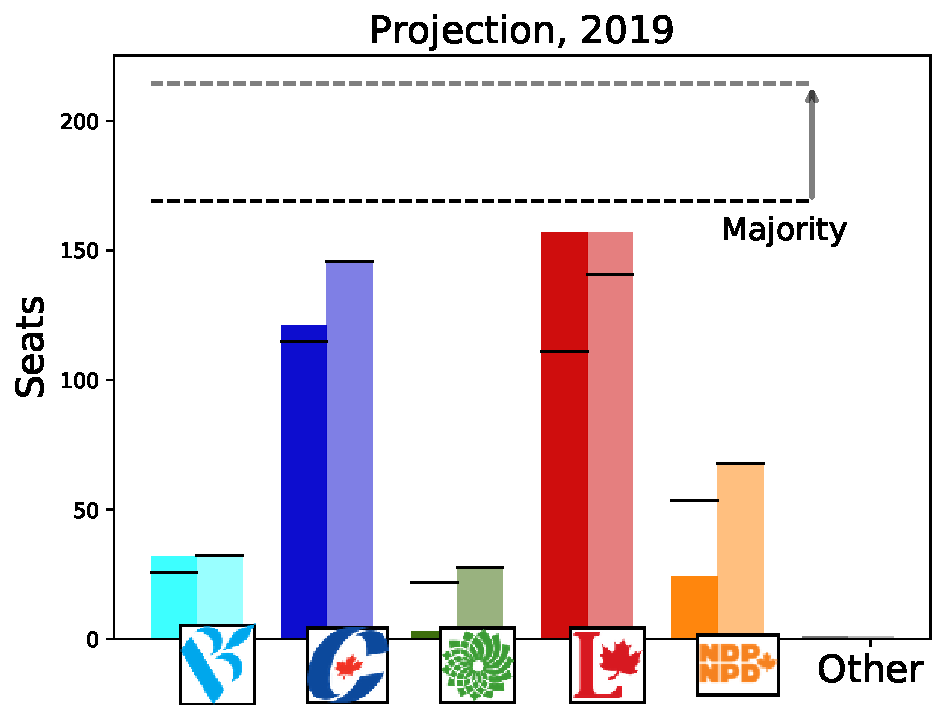
\includegraphics[width=0.50\textwidth,clip]{PR_calcs/data/raw_2019/PMM_out/PMM_projections.pdf}
  \caption{Projected seat distribution following the 2019 federal election, using actual results (left) alongside projected results of this model from the same electorate in transparency (right). The dashed line denotes majority control for both cases, while a finer black line for each party shows the number of seats that would correspond to their share of the popular vote. PMM leaves no party underrepresented, but allows \emph{over}-representation to be partially preserved (albeit, reduced), which incentivises riding-level contests.}
\label{fig:sum_projection_2019}
\end{figure}
